\documentclass[jair,twoside,11pt,theapa]{article}
\usepackage{jair, theapa, rawfonts, graphicx, color, caption, amsmath}

%\jairheading{1}{2018}{}{}{}
\ShortHeadings{Distributed Q-Learning (DistQL)}
{Robinson}
\firstpageno{1}

\begin{document}

\title{Distributed Q-Learning: A Democratic Learning Process}

\author{\name Max Robinson \email max.robinson@jhu.edu \\
       \addr Johns Hopkins University,\\
       Baltimore, MD 21218 USA
   }

% For research notes, remove the comment character in the line below.
% \researchnote

\maketitle

\begin{abstract}

\end{abstract}

\section{Introduction}
\label{Introduction}
Reinforcement learning can be described simply as the learning process of an agent in an environment trying to reach a goal. 
The agent learns by attempting to maximize a reward. In some situations the learner has very little prior knowledge of the environment. 
The act of maximizing the reward is the learning process.

Reinforcement learning typically requires an agent to follow a $state \to action \to state'$ loop. As a result, the learning process is also typically sequential. 
For large state spaces or complex environments, this process can be slow. A single agent must often experience many iterations of maximizing 
a reward in order to learn in even a simple environment.

A famous example of Reinforcement Learning is Tesauro's TD-Gammon agent.
The best performing agent required 1,500,000 training games to beat one of the best Backgammon players at the time \cite{Tesauro:1995:TDL:203330.203343}.
As a more modern example, Mnih et al. (2013) \nocite{Mnih2013} developed an algorithm to play Atari 2600 video games called DQN. To learn to play each game at a human level or higher,
50 million frames were required to train an agent for each game. Total training on all 49 games in the study took about 38 days of game experience (Mnih et al. 2015). 

The constraint of a lone agent acting sequentially can create situations where training an agent to learn a task can take an exorbitant number of episodes. 
To combat this, researchers have focused on ways to adapt these reinforcement learning algorithm to run in parallel to decrease the number of episodes it takes for a single agent to achieve high performance.
%a single agent to learn. 

Recent research has studied speeding up Deep Neural Networks for reinforcement learning such as DQN (Mnih et al., 2013)\nocite{Mnih2013} and others. Quite a few papers have suggested ways of parallelizing both the computation for these methods as well as distributing actors and learners to run in parallel, which send back gradients to be used to update a centralized parameter store. 

%This proposal suggests a step back to explore a slightly more simplistic model of distributed reinforcement learning using Q-learning. It suggests a parallelized and distributed version of the Q-learning algorithm using a traditional Q-memory, hereon in referred to as Distributed Q-learning (DistQL). DistQL, similar to other distributed reinforcement learning approaches, uses multiple separate agents and environments with local copies of parameters and memory to learn, and has a centralized main Q-memory. Different from other algorithms, however, DistQL sends learned Q-values to the centralize memory which are then combined with the existing values. The centralized Q-memory then updates values, using a linear combination of Q-values and hyperparameters explained in Section \ref{Approach}. An advantage to this approach is that the traditional Q-learning algorithm is being leveraged. This means that the optimality convergence guarantees of Q-learning, even in an asynchronous settings, are likely to still hold true.


\section{Previous Work}
\label{Literature Survey}
Q-Learning \cite{watkins} has been a foundational algorithm in reinforcement learning, especially after it was shown to have optimal convergence in the limit \cite{qlearning}. Very soon after this, asynchronous methods of Q-learning were being explored.  

Tsitsiklis (1994) \nocite{Tsitsiklis1994} studied if Q-learning would still keep its optimal convergence property in an asynchronous setting. The results showed that the Q-learning algorithm does continue to keep this convergence guarantee in an asynchronous setting, given that old information is eventually discarded through the update process, along with a few other conditions. 

More recently there has been a flurry of work done in parallelizing reinforcement learning algorithms. Mannion, Duggan, \& Howley (2015) \nocite{MANNION2015956} used a distributed Q-learning algorithm with multiple agents and environments to learn in, applied to traffic signal control. In their algorithm, at every time step the agents update a global Q Matrix in accordance with the Q-learning update equation. 

In addition to using a tabular implementation of Q-learning, function approximation versions using deep neural networks, such as DQN (Mnih et al., 2013), have also explored asynchronous and distributed architectures for learning. 

The General Reinforcement Learning Architecture (Gorila) (Nair et al. 2015)\nocite{Gorila} uses a general, massively distributed architecture of agent, and environments to learn. Each agent in Gorila has its own environment, a copy of the model which is periodically updated, a separate replay memory and a learner that aims to learn using a DQN (Mnih et al., 2015)\nocite{Mnih2015}. The learner samples data from the memory replay and computes the gradients for the parameters, which are then sent to a centralized parameter server. The parameter server then updates a central copy of the model based on gradients. 

A3C (Mnih et al. 2016)\nocite{A3C} collapses Gorila onto a single machine, using multiple processors to parallelize the agents actions in an environment. A3C similarly computes gradients for each agent's model at each time step, locally, but accumulates these gradients over a series of time steps before updating the central model, every so often. This aims to balance computational efficiency with data efficiency. 

\section{Q-Learning}
\label{Q-Learning}

\section{Distributed Q-learning} 
\label{algorithm}
Distributed Q-Learning (DistQL) uses Q-Learning as a foundation for learning and delegates learning to multiple agents, similar to what is done in A3C and Gorilla. DistQL uses multiple worker agent-environment pairs to learn rather than a single agent and environment. As the agents learn and complete epochs, a central QServer, with memory $Q_c$, is updated. The QServer is updated at regular intervals by the workers, based on an update frequency $\tau$. The QServer also keeps a central learning rate $\eta_{c,(s,a)}$ for each $(s,a)$ pair. This learning rate is decayed according the the number of times that particular $(s,a)$ pair has been updated. 

More formally, DistQL has $n$ worker agents $A_1,..., A_n$. Each agent also has a copy of the environment in which it acts, $E_1,...,E_n$. Each agent keeps track of a local Q-memory, $Q_i$, as well as local parameters such as discount factor $\gamma_i$, exploration chance $\epsilon$, and learning rates $\eta_{i,(s,a)}$. Each agent acts and learns inside of its environment according to an $\epsilon$-greedy Q-Learning algorithm.

As the worker learns it will send updates to the QServer, $Q_c$. In order to send updates, a list of $Q_i(s,a)$'s that have been modified since the agent last sent an update is kept by the worker, $Set_{Q_i} = Set(Q_i'(s,a),...)$. The agent sends updates to $Q_c$ every $\tau$ epochs. $\tau$ is a hyperparameter that can be adjusted to change the frequency with which workers update $Q_c$. An architecture digram of DistQL can be seen in Figure \ref{fig:DistQLArchitecture}. 

\begin{figure}[h]
\centering
\includegraphics[width=0.8\linewidth]{"DistQL Architecture-modified"}
\caption{DistQL Architecture with 4 agents}
\label{fig:DistQLArchitecture}
\end{figure}

The QServer updates $Q_c$ each time it receives an update from a worker. $Q_c$ is updated in accordance to equation 1. For readability $\eta_c$ is used for brevity with the understanding that the learning rate is actually $\eta_{c,(s,a)}$.

\begin{equation}
\label{eq1}
Q_c(s,a) = (1-\frac{\eta_{c}^{2}}{\eta_{i}})Q_c(s,a) + \frac{\eta_{c}^{2}}{\eta_{i}} Q_i(s,a), \text{  } 0 < \eta_{c} \leq \eta_{i} < 1
\end{equation}

Equation \ref{eq1} can also be thought of as an aggregation function of worker Q-values. It is built on the idea that the learning rate $\eta$ can be thought of as a measure of how certain the algorithm is that the current Q-value stored will be the final Q-value in the table. For instance, if $\eta_{i,(s,a)} = .9$ and $Q_{i,(s,a)} = 1$ the worker will apply a large learning rate on the next update to $(s,a)$. This means that the worker is willing to make larger adjustments to the Q-value, and it is less likely that the current Q-value will be the same as the final Q-value in the table, compared to later on. If $\eta_{i,(s,a)} = .01$ and $Q_{i,(s,a)} = 1$, it is much more likely that the current Q-value for $(s,a)$ will remain close to the current Q-value. 

The ratio $\frac{\eta_{c}^{2}}{\eta_{i}}$ is calculated to quantify how much the worker $i$ and $Q_c$ agree about how stable the Q-value in $Q_c$ is. The ratio can be re-written as $\frac{\eta_{c}}{\eta_{i}} \eta_{c}$ to demonstrate this more clearly. If $\eta_{c} = \eta_{i}$ then $Q_c$ and $Q_i$ agree on how stable the Q-value is, and an update of $(1-\eta_{c})Q_c + \eta_{c} Q_i(s,a)$. Otherwise, $\frac{\eta_c}{\eta_i} < 1$ which puts more emphasis on the Q-value already stored by $Q_c$ rather than $Q_i$. Intuitively, the idea is that if the central Q-value is more stable than a workers, then the central value should not be highly impacted by a worker's value which is less likely to converge to its own Q-value.

It is possible for $\eta_i$ to be less than $\eta_c$ when updates are sent to the QServer. One case where this can happen is if the worker has updated a local $(s,a)$ more times than $Q_c$ has updated $(s,a)$. When $\eta_i < \eta_c$, the central learning rate adopts the workers learning rate such that $\eta_c \leftarrow \eta_i$ prior to the update taking place. This ensures that the central learning rate is always less than or equal to the workers learning rate. Since the learning rate is interpreted as a measure of stability for the Q-value, if a worker has a Q-value that is more stable than the central server, the server wants to acknowledge and adopt the learning rate of the worker, when updating $Q_c$.

%This also allows for workers have differing ideas about the stability of different Q-values. The QServer is then the arbiter of these ideas, and reconciles the difference based on a central learning rate. 

%A central learning rate $\eta_c$ is used for a few different reasons. 
Using a central learning rate $\eta_c$ allows for the update equation to remain asynchronous. By keeping a central learning rate, the QServer can remain agnostic to the frequency of the updates from workers and from the order of the updates. This means less logic must be written to coordinate the updates from workers. This allows each worker to update the $Q_c$ without having to wait for other workers to also be updating $Q_c$. This also means that, not all workers have to be started at the same time, or remain in-sync with other works on which epoch they are on. This has benefits from a scaling perspective since allows workers to be far less dependent on the QServer. 

% talk about updates pushed back to workers. 
After updates to $Q_c$ are made, there are two strategies that are explored for updating the workers. The QServer can either send the entire contents of $Q_c$ to the worker, or it can send back only updates states that the worker initially sent to the QServer. These options are denoted DistQL-ALL and DistQL-Partial respectively. DistQL-ALL is the default option, and is synonymous with DistQL. 

In DistQL-ALL, workers will receive the response from the QServer which contains a copy of $Q_c$. The worker will then overwrite all $Q_i$ Q-values with the corresponding $Q_c$ Q-value. For any states in $Q_c$ that are not in $Q_i$, the agent adopts both the Q-value and the learning rate from $Q_c$. This method provides workers with additional information collected from other workers and has the effect of homogenizing their memories. In this variation, state-action pairs that were explored by one worker would then be shared with other workers even if the worker has not explored that state-action pair.

In DistQL-Partial, workers only receive updates for the states submitted to the QServer. If worker $A_i$ updates the QServer with $Set_{Q_i}$, $A_i$ receives back a set $Set_{Q_i}'$ containing the same set of state-action pairs but with Q-values from $Q_c$. The worker then replaces any local Q-values with values in the response set. This adaptation just has the effect of reconciling the Q-values known by the worker with the central server. This provides shared knowledge only about states the worker knows about. No new state-action pairs are shared through this update. Thus exploration is not shared across workers. 



\section{Experiments}
\label{experiments}
To demonstrate the effects of DistQL, the Taxi world \cite{Dietterich2000} and Cart Pole (Barto et al. 1983)\nocite{Barto83} environments were chosen for agents to learn in. The environment implementations used are part of the OpenAI Gym \nocite{gym} and are publicly available. The goal in each environment is for the agent to achieve the highest reward possible in the environment. 

The taxi world is a 5 by 5 grid world where the agent is a taxi driver, and there 4 marked spaces in the grid. The goal of the agent is to navigate to the passenger, pick him or her up, navigate to the goal, and drop the passenger off at another destination. For rewards, the agent receives +20 points for successfully dropping off the passenger, -1 point for every time step, and -10 penalty for any illegal pick-up or drop-off actions made. The actions available to the agent are to move in the four cardinal and perform a pick-up or drop-off action. An episode finishes after the passenger has been successfully dropped off at their destination.

The Cart Pole environment consists of trying to balance a pole upright while attached by a joint to a cart on a frictionless track. The pole starts upright and the goal is to keep the pole balanced upright for as long as possible. The cart can move left or right along the track by applying a force of +1 or -1. The episode finishes after the pole leans 15 degrees left or right or the cart has moved 2.4 units from the center. A reward of +1 is given to the agent for every time step that the pole stays upright. For this experiment, the OpenAI implementation was modified so that when an episode is terminated a reward of -200 is incurred. 

For Cart Pole, the implementation uses a continuous state space with 4 features. In order to apply Q-Learning, the continuous state space must be discretized. The first three features are discretized into 8 bins of equal size, with values between -2.4 to 2.4, -2 to 2 and -1 to 1 for features 0, 1, and 2 respectively. The fourth feature is discretized into 12 bins of equal size between the values of -3.5 to 3.5. This specific discretization is chosen because of the anecdotal and demonstrated success described by Victor Vilches (2017)\nocite{Victor:github}. 

A series of experiments were run in each environment. DistQL-ALL and DistQL-Partial were run with 1, 2, 4, and 8 agents each with 10 trials. Each trail consists of 2000 epochs for each agent. A limit of 2000 epochs per trail is used to allow for reasonable training times on a smaller machine but still demonstrate learning occurring in each environment. For each number of agents run, $\tau$ was adjusted to be 10, 50, and 100. This allows a comparison of how update frequency impacts learning. Table 1 shows all experiments performed. A total of 48 experiments were run. 
%% Talk about \tau here. 

Each agent and the central Q server used the same hyperparameters for all experiments. The learning rate $\eta$ for each $(s,a)$ was initialized to .5 and decayed so that $\eta = 0.5 \times 0.999^i$ where $i$ is the $ith$ update to $(s,a)$. The exploration rate $\epsilon$ was initialized to .1 and decayed so that $\epsilon = 0.5 \times 0.999^j$ where $j$ is the $jth$ episode in the learning process. The discount factor $\gamma$ was set to .9. These hyperparameters were chosen based on anecdotal success of a single Q Learner acting in the environments. An exhaustive search for optimal hyperparameters and decay rates was not performed. 

\begin{figure}[h]
\centering
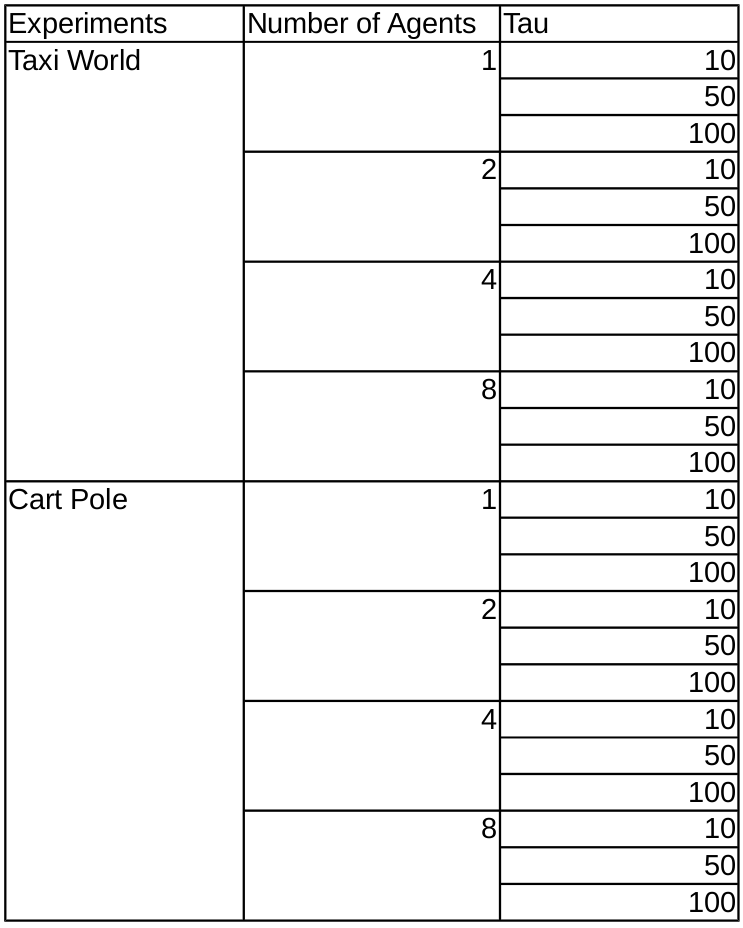
\includegraphics[width=0.7\linewidth]{ExperimentTable}
\caption*{Table 1: Experiment Table}
\label{fig:ExperimentTable}
\end{figure}

% Talk about source code
For these experiments, the DistQL was implemented in Python 3.5 using an http-based client-server architecture. Each agent was run in a thread and provided updates and received responses through the http protocol. The server implementation is single-threaded and does not allow for concurrent modification of the Q-memory. The Q-Learning agent is also written in python as part of a framework for DistQL. All source code for the DistQL implementation can be found at https://github.com/MaxRobinson/DistributedQMemory.

\subsection{Evaluation} 
\label{evaluation}
Since in each environment gives a reward at each time step, the cumulative reward for each episode is used to judge the performance of the agent or agents in each environment. Specifically, the average cumulative reward for each set of agents over the 10 trails is compared with each other set of agents in that environment. For example, the performance of DistQL-ALL with 2 agents is calculated by taking the average cumulative reward for each epoch that each agent experienced over the 2000 epochs individually, and then averaging the performance of the two agents together. This provides an aggregate average cumulative reward for all agents in DistQL-ALL for 2 agents. 

The performance of the DistQL with the different number of agents are compared to one another. A set of agents is considered to have done better if the average cumulative reward achieved by the set of agents is higher than other sets of agents earlier on. The higher the average cumulative reward achieved earlier, or in fewer episodes, the better.

\section{Results and Analysis}
\label{results}
The results of the experiments provide insight into the performance of sets of agents when compared to each other in the same environment. In addition, the results show how the update method for DistQL and the update frequency can effect learning performance. The first environment examined is the Taxi World. 

Figure \ref{fig:DistQL-ALL-tau-10-env-Taxi} compares the performance of each set of 1, 2, 4, and 8 agents to each other using DistQL-ALL, based on average cumulative reward. The figure shows that as the number of agents increased, fewer episodes were require for each agent to reach a higher cumulative reward. There is an almost linear decrease of $\frac{1}{\# agents} \times \text{number of episodes required}$ for each agent. This suggests that when running a set of 8 agents with DistQL-ALL, each agent would only need to perform about 1/8th the number of episodes to reach the same performance of a single learning agent. The figure also illustrates how much faster the set of 8 agents was able to converge to an optimal policy when compared to the other sets of agents.

\begin{figure}[h]
\centering
\begin{minipage}{.5\textwidth}
	\centering
	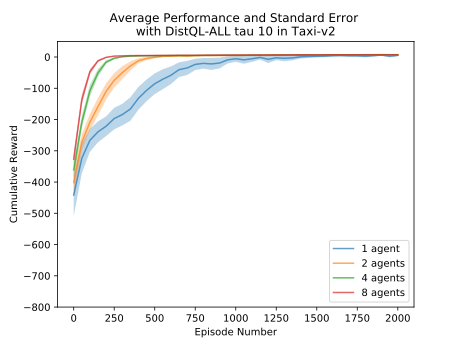
\includegraphics[width=1\linewidth]{resultImages/binned-Average-Performance-and-Standard-Error-with-DistQL-ALL-tau-10-in-Taxi-v2}
	\caption{}
	\label{fig:DistQL-ALL-tau-10-env-Taxi}
\end{minipage}%
\begin{minipage}{.5\textwidth}
	\centering
	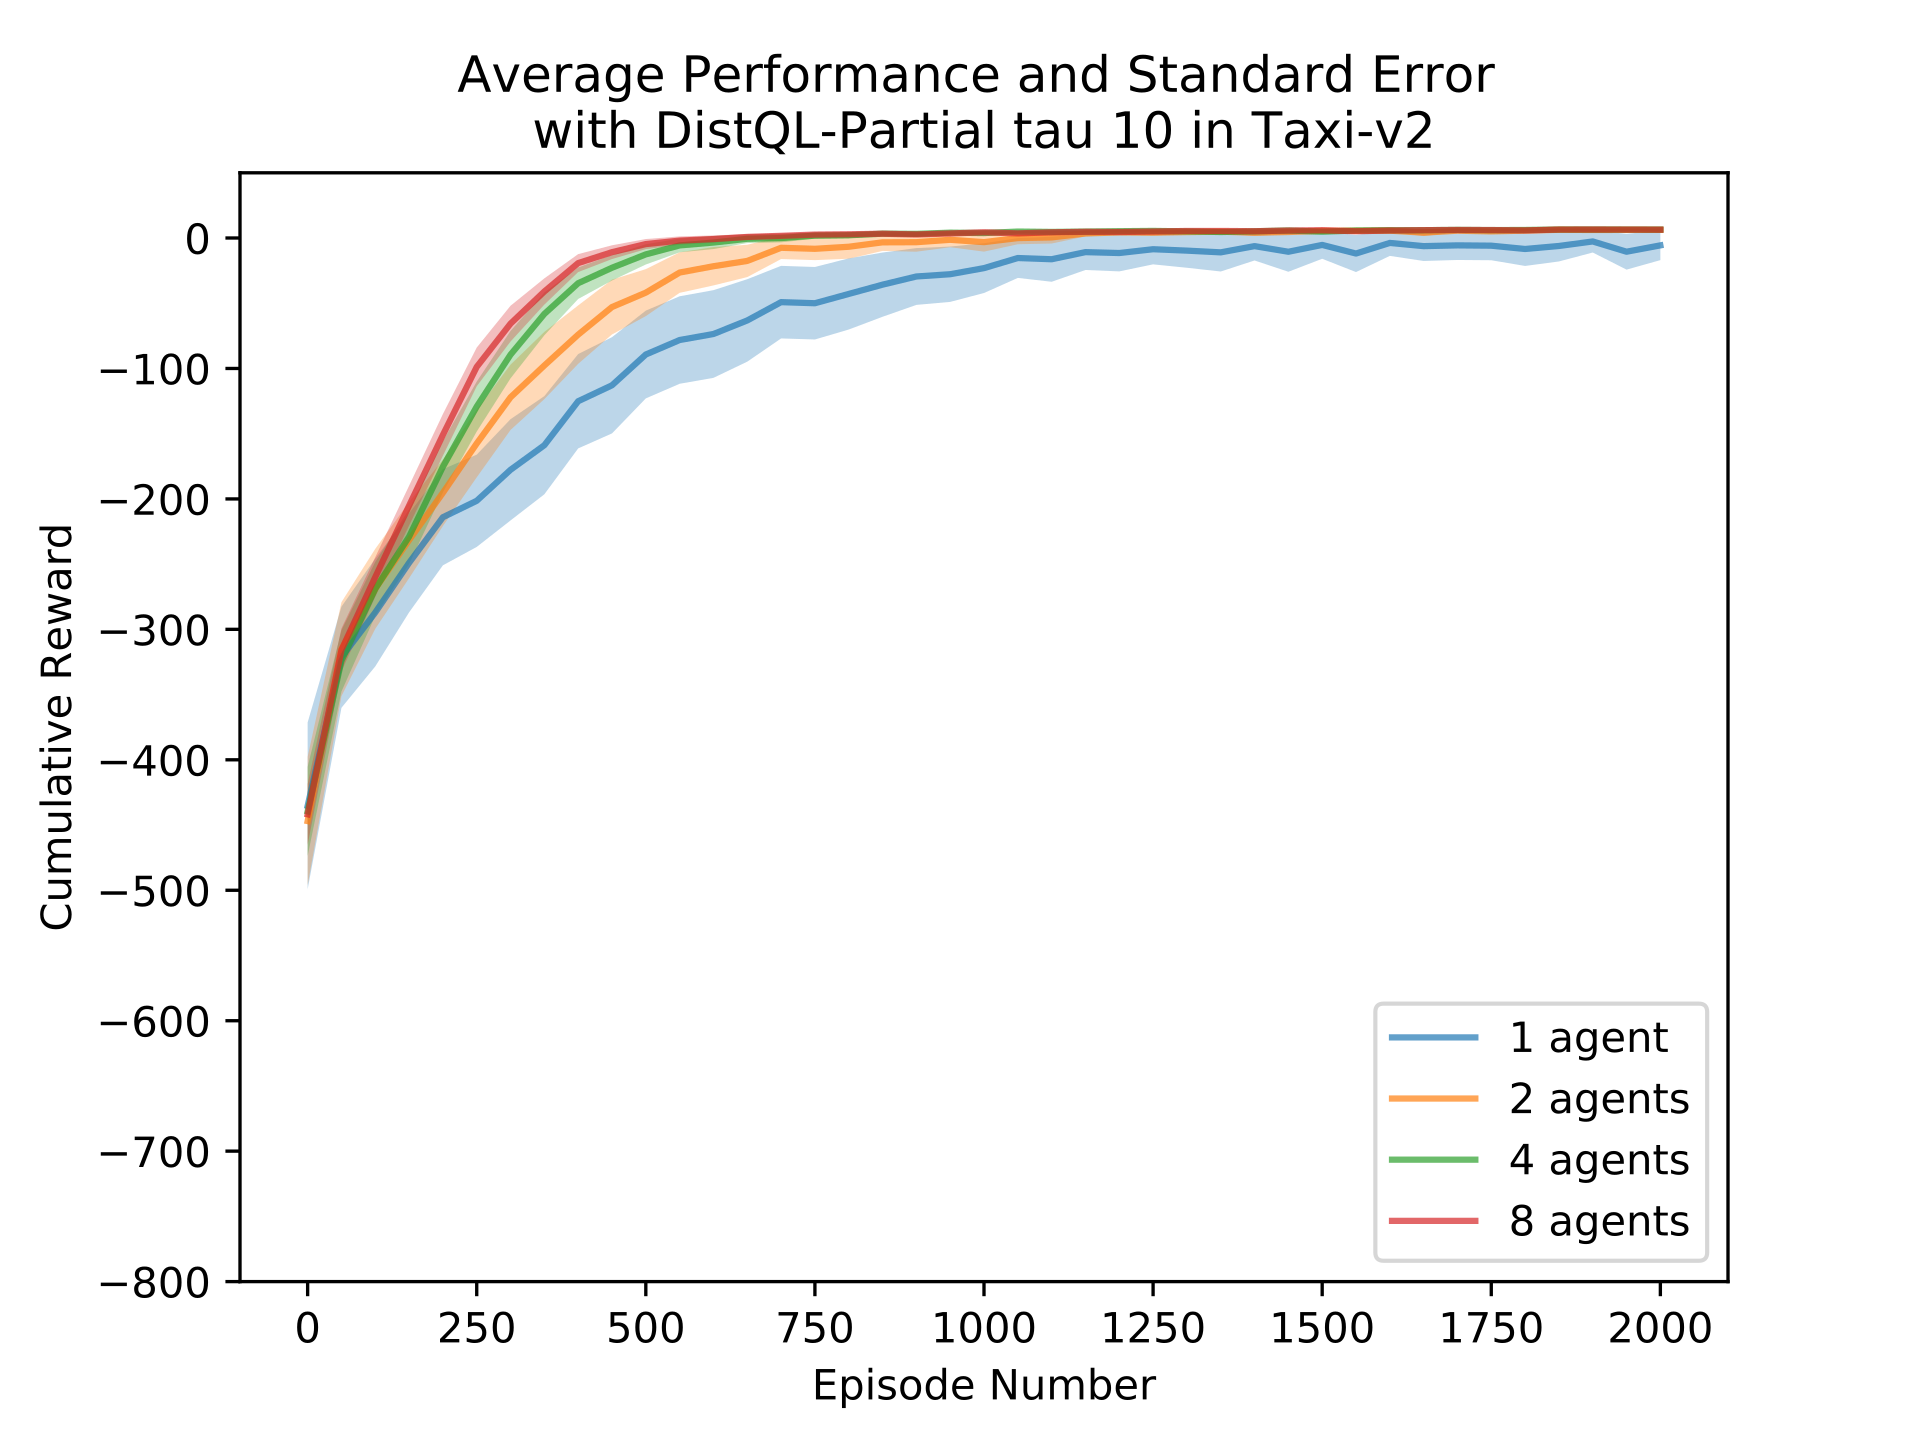
\includegraphics[width=1\linewidth]{resultImages/binned-Average-Performance-and-Standard-Error-with-DistQL-Partial-tau-10-in-Taxi-v2}
	\caption{}
	\label{fig:DistQL-Partial-tau-10-env-Taxi}
\end{minipage}
\end{figure}

Figure \ref{fig:DistQL-Partial-tau-10-env-Taxi} shows the performance when the DistQL update method is changed to DistQL-Partial. There is still an increase in the rate of performance as the number of agents per set increases, but it is less pronounced. The agents all take a little longer to learn in the beginning and then start to differentiate after that. This suggests that the first part of the learning process is each agent exploring. After more and more states are discovered, the aggregation of the value of the explored states helps to give the sets with more agents a boost in learning. This suggests that a large part of the success of DistQL-ALL is due to the agents shared exploration in combination with the aggregated Q-values. 

The Cart Pole environment showed similar but less straight forward results. As in the Taxi world, Figure \ref{fig:DistQL-ALL-tau-10-env-CartPole} shows an initial increase in performance as the number of agents in a set increases. However this, increase is less pronounced, and as the number of episodes elapsed increases, these performance gains decrease. The use of 4 or 8 agents in this world is especially less pronounced than in the Taxi world. 

\begin{figure}[h]
	\centering
	\begin{minipage}{.5\textwidth}
		\centering
		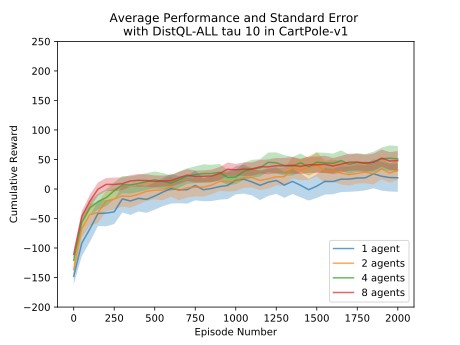
\includegraphics[width=1\linewidth]{resultImages/binned-Average-Performance-and-Standard-Error-with-DistQL-ALL-tau-10-in-CartPole-v1}
		\caption{}
		\label{fig:DistQL-ALL-tau-10-env-CartPole}
	\end{minipage}%
	\begin{minipage}{.5\textwidth}
		\centering
		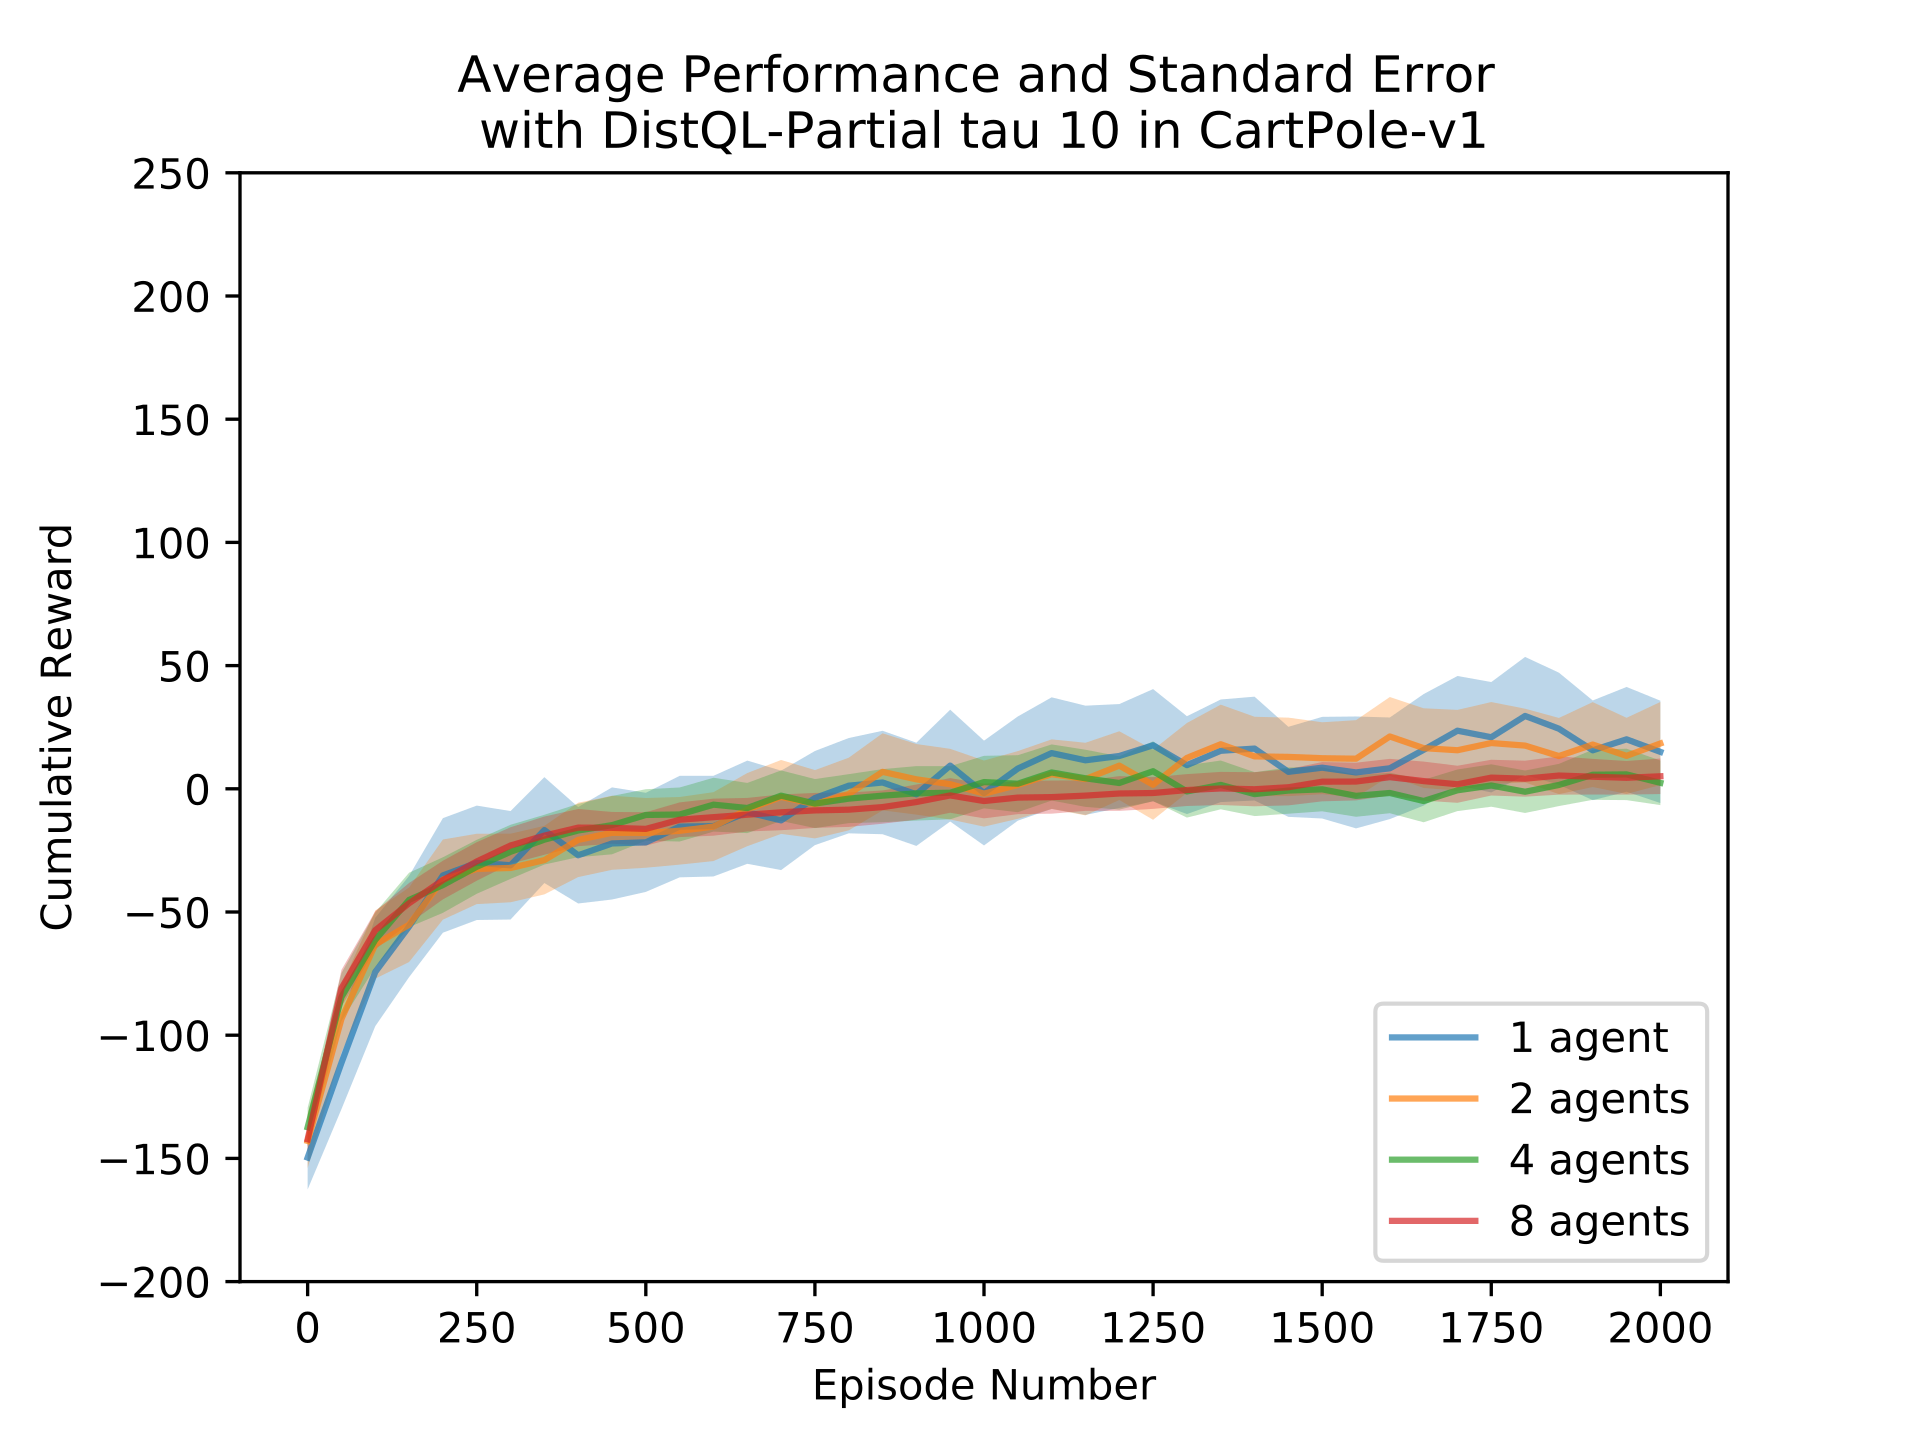
\includegraphics[width=1\linewidth]{resultImages/binned-Average-Performance-and-Standard-Error-with-DistQL-Partial-tau-10-in-CartPole-v1}
		\caption{}
		\label{fig:DistQL-Partial-tau-10-env-CartPole}
	\end{minipage}
\end{figure}

For DistQL-Partial, the performance looks much more like each set were just individual agents. The benefit of having more agents does not seem to have much positive effect. This is most likely due to the agents not being able to find the same state-action pairs early on to then communicate with other agents. In fact, it seems almost the reverse, while towards the maximum number of episodes the average behaviors of each set are similar, the standard error for the set with only 1 agent shows that it is consistently able to reach higher scores than the set with 8 agents, though the mean performance is about the same. This helps demonstrates the power of sharing exploration experience. 

Next, the effect of changing the update frequency $\tau$ is shown. DistQL-ALL is used to demonstrate the effect since the results were similar and DistQL-ALL performed better in all situations. In the Taxi world, shown in Figure \ref{fig:DistQL-ALL-tau-50-env-Taxi} and Figure \ref{fig:DistQL-ALL-tau-100-env-Taxi}, the number of episodes required to achieve the same cumulative reward as with $\tau=10$ starts to increase. This make sense since information is being shared less frequently. The decrease in the frequency of information sharing increases the time it takes to aggregate the information.
\begin{figure}[h]
	\centering
	\begin{minipage}{.5\textwidth}
		\centering
		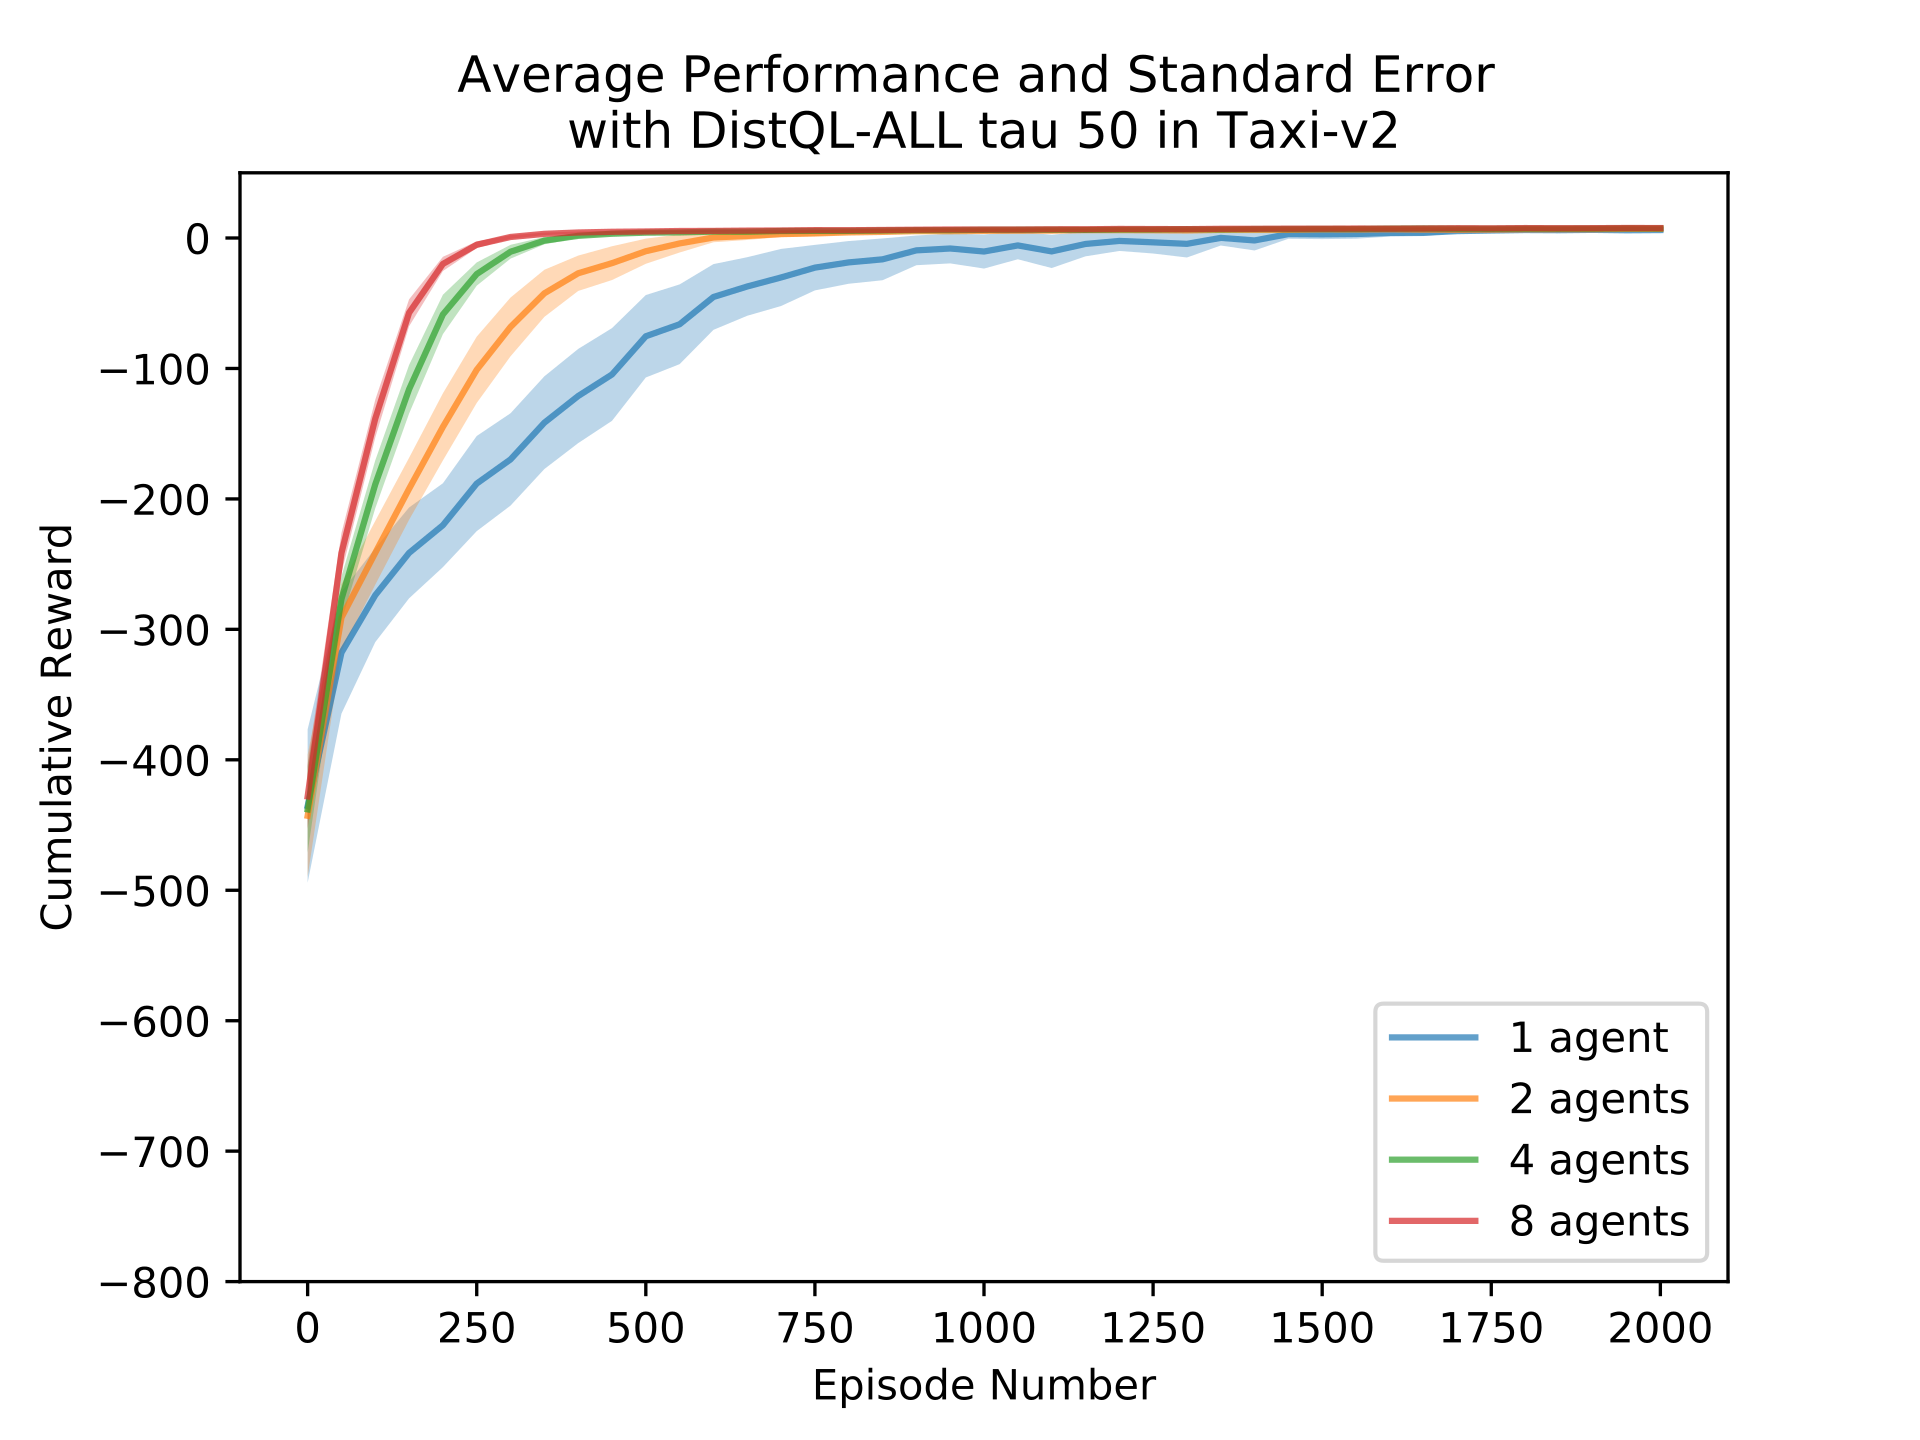
\includegraphics[width=1\linewidth]{resultImages/binned-Average-Performance-and-Standard-Error-with-DistQL-ALL-tau-50-in-Taxi-v2}
		\caption{}
		\label{fig:DistQL-ALL-tau-50-env-Taxi}
	\end{minipage}%
	\begin{minipage}{.5\textwidth}
		\centering
		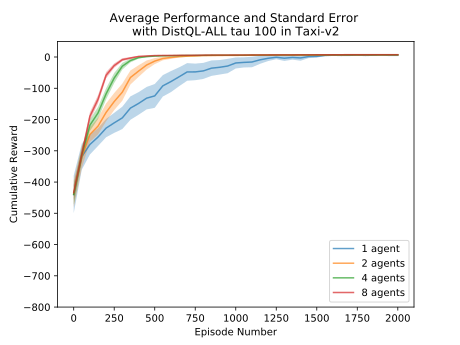
\includegraphics[width=1\linewidth]{resultImages/binned-Average-Performance-and-Standard-Error-with-DistQL-ALL-tau-100-in-Taxi-v2}
		\caption{}
		\label{fig:DistQL-ALL-tau-100-env-Taxi}
	\end{minipage}
\end{figure}%
\begin{figure}[h]
	\centering
	\begin{minipage}{.5\textwidth}
		\centering
		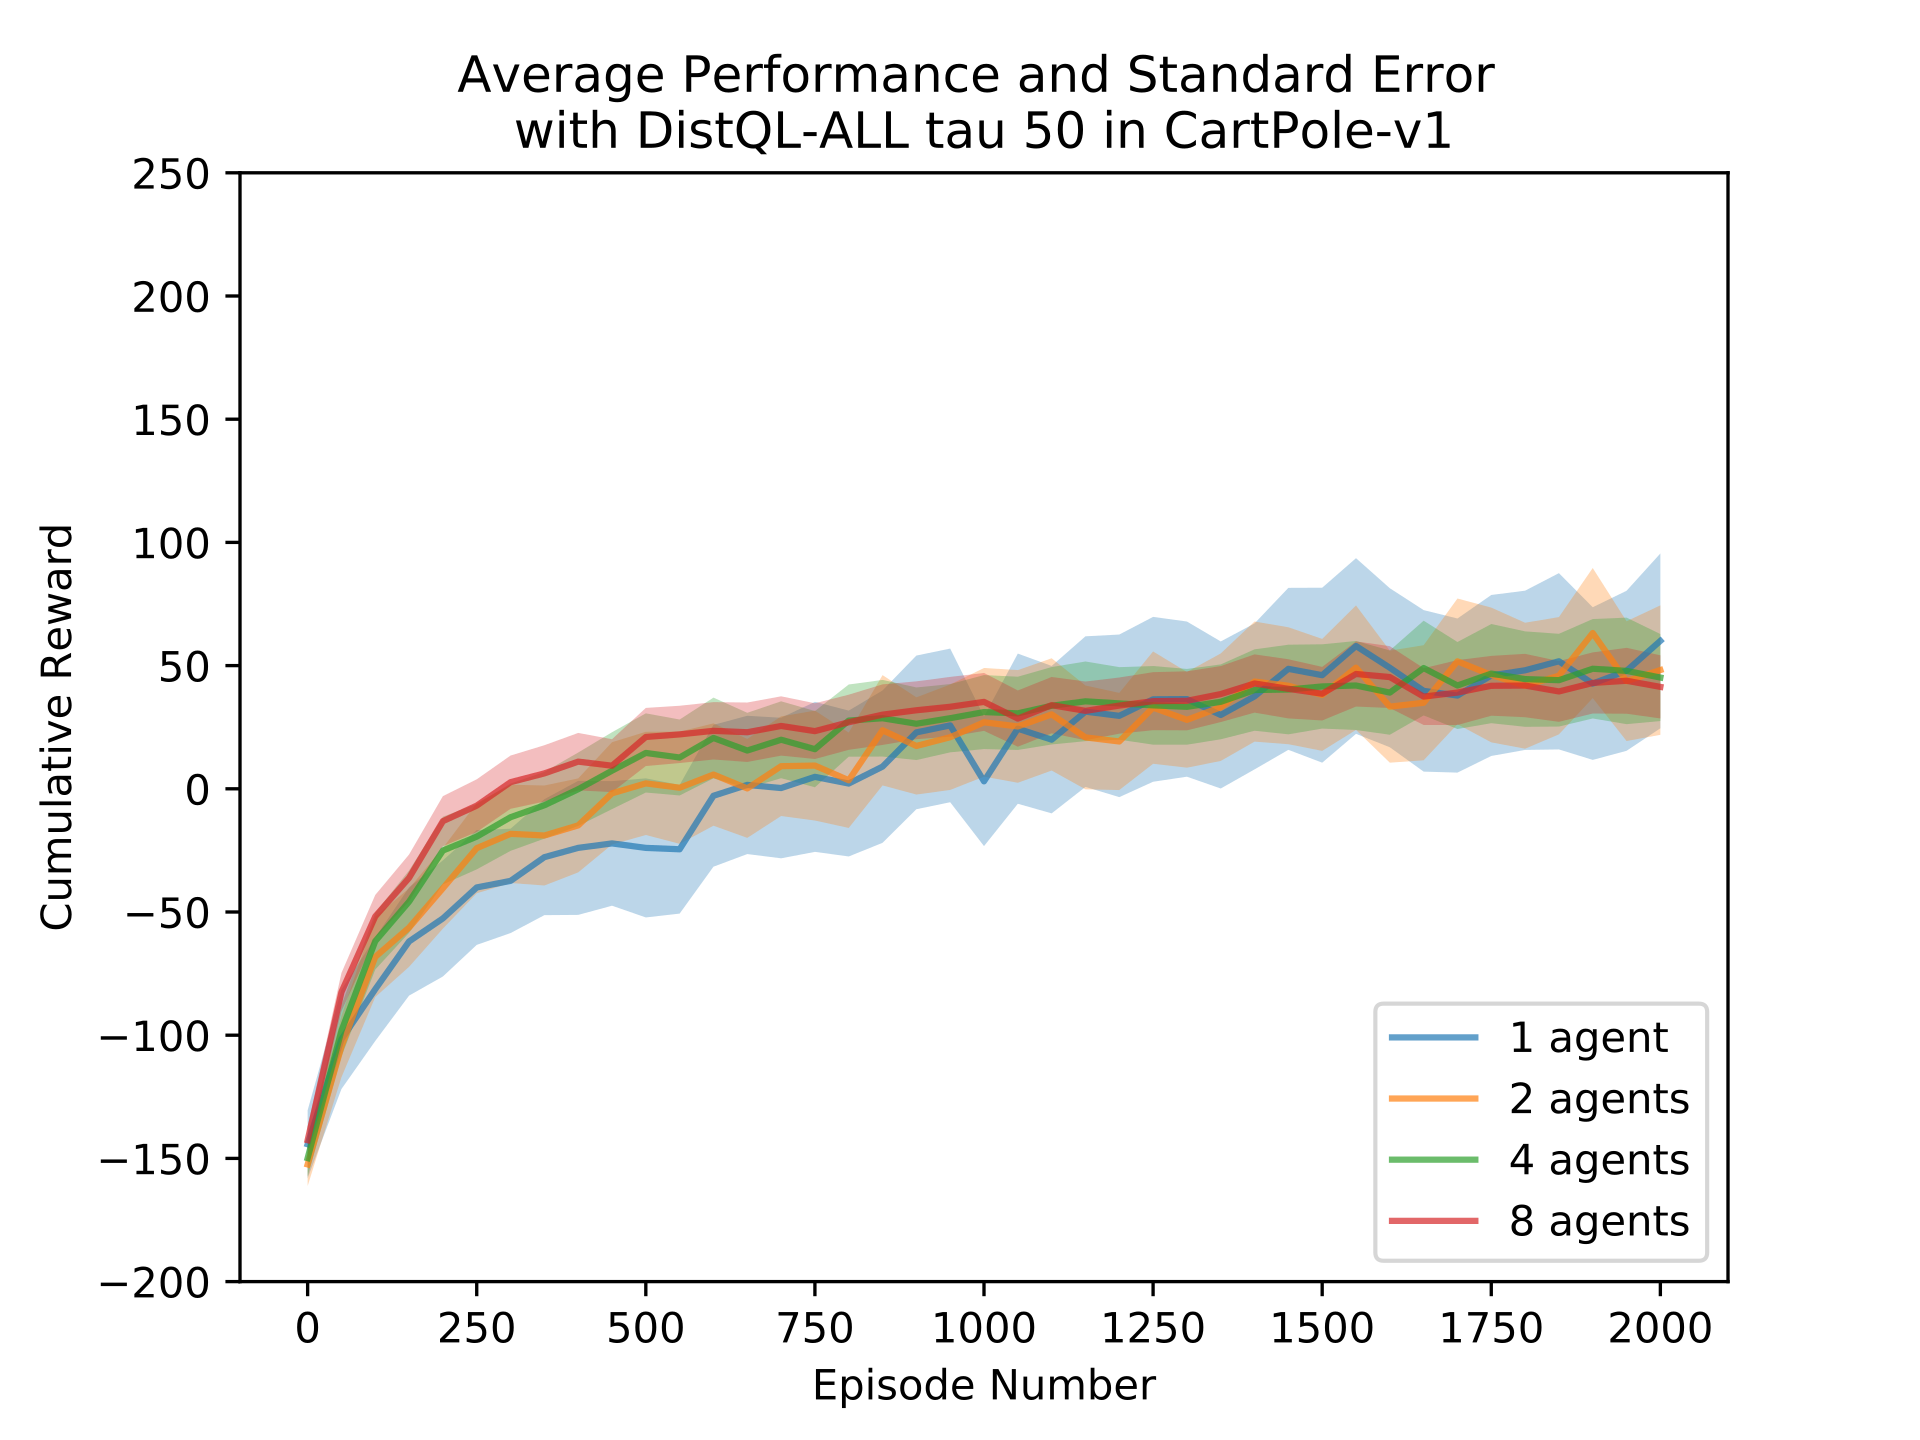
\includegraphics[width=1\linewidth]{resultImages/binned-Average-Performance-and-Standard-Error-with-DistQL-ALL-tau-50-in-CartPole-v1}
		\caption{}
		\label{fig:DistQL-ALL-tau-50-env-CartPole-v1}
	\end{minipage}%
	\begin{minipage}{.5\textwidth}
		\centering
		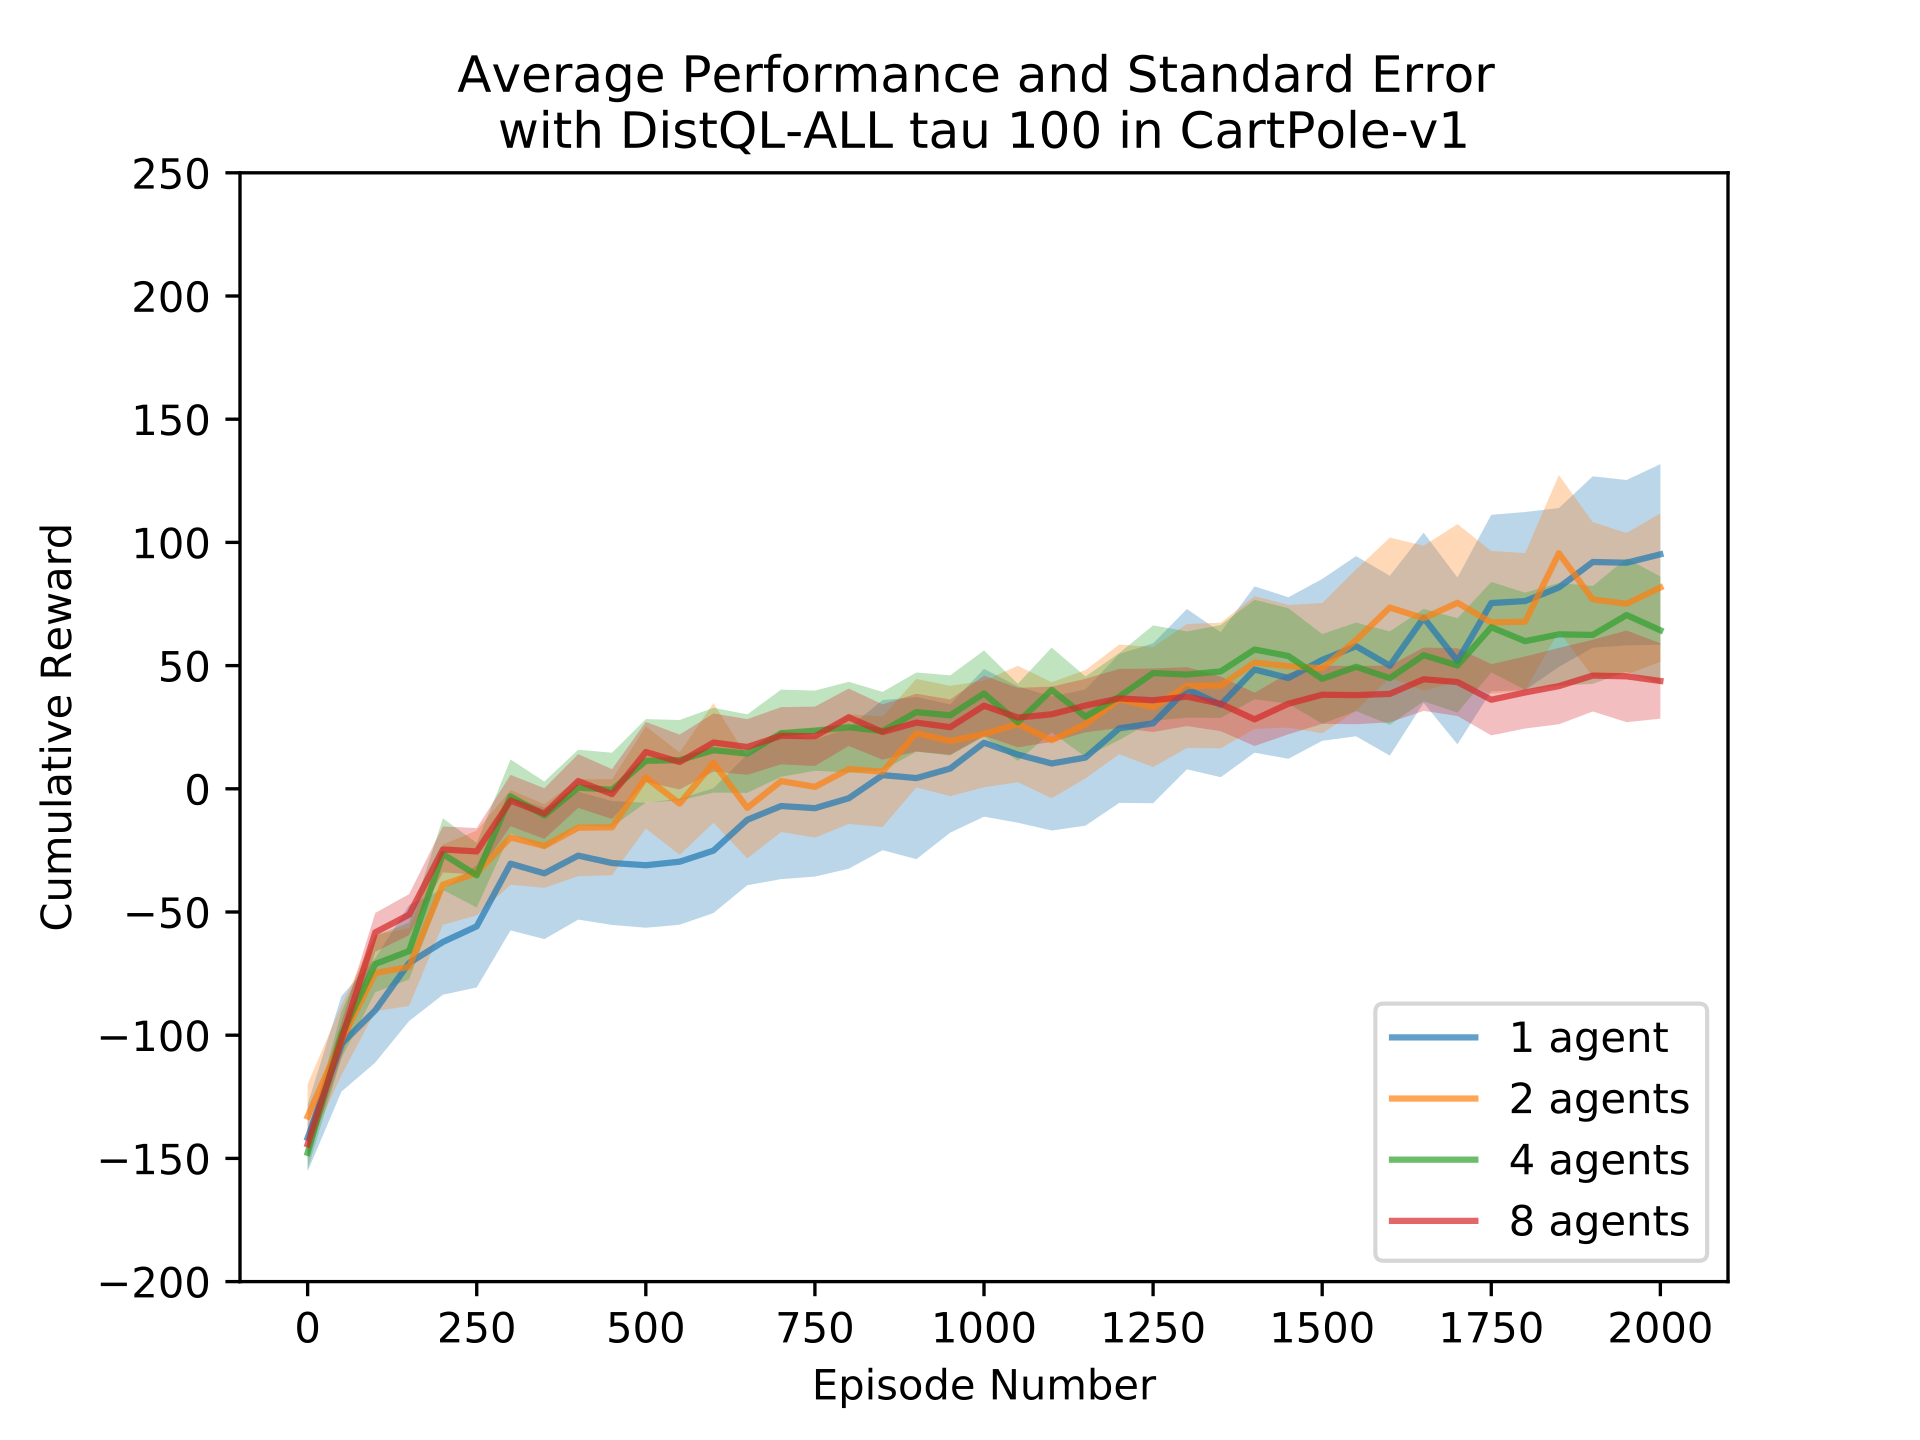
\includegraphics[width=1\linewidth]{resultImages/binned-Average-Performance-and-Standard-Error-with-DistQL-ALL-tau-100-in-CartPole-v1}
		\caption{}
		\label{fig:DistQL-ALL-tau-100-env-CartPole-v1}
	\end{minipage}
\end{figure}

The same effect can be seen early on in the Cart Pole Environment. It takes more episodes to reach the same early cumulative reward as with an update frequency of 10 early on. Interestingly, an increase in the update frequency had a slightly different effect as training continued with an update frequency of 100. As the number of episodes elapsed increased, the sets of agents with 1, 2, of 4 agents seemed to do better, while 8 agents performed about the same. 

This is believed to happen for two reasons. One, is that there is high variance in the environment. Since the environment is initially continuous and had to be discretized, there is possible ambiguity in what values are learned for the states. This could lead to high variance in learning the value for a state-action pair across training sets. The second is that the learning rate is competing with the exploration for this environment. As the number of updates becomes more infrequent, the central learning rates are decayed less often. In addition, as the number of agents decreases the number of times the central learning rates decay decreases. This would be important if agents are still exploring more episodes into the learning process. The decay rate of the learning rates on the QServer is not scaled based on the number of agents involved. This would help explain why the performance of 8 agents seemed to be more constant across values of $\tau$ than 2 agents.

To possibly fix the second issue, different hyperparameters could be found for the Cart Pole environment. The learning rate and decay would accommodate for the larger amount of exploration needed to find an optimal policy. The suspected reason why this result was seen with Cart Pole and not the Taxi world is due to the difference in state space size and reward shaping. The Taxi world has about  $2.4 \times 10^8$ number of state-action pairs, but due to the reward shaping, agents tend to quickly learn not to make illegal drop-off and pick-up moves. This tends to decrease the effective size of the state space. In comparison there is little reward shaping for Cart Pole. With the discretization used the state space is about  $3.7 \times 10^7$ state-action pairs. Cart Pole might require a longer exploration period than the Taxi world. Again, this can likely be addressed through the hyperparameters for the learning process. 


\iffalse

\begin{figure}[h]
	\centering
	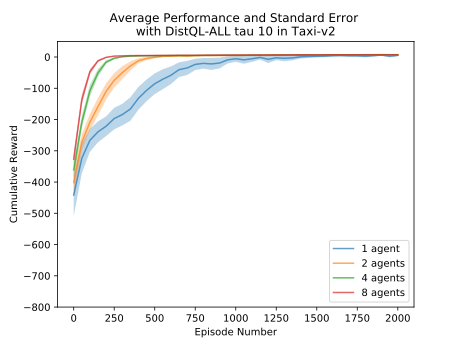
\includegraphics[width=1\linewidth]{resultImages/binned-Average-Performance-and-Standard-Error-with-DistQL-ALL-tau-10-in-Taxi-v2}
	\caption{}
	\label{fig:binned-Average-Performance-and-Standard-Error-with-DistQL-ALL-tau-10-in-Taxi-v2}
\end{figure}

\begin{figure}[h]
	\centering
	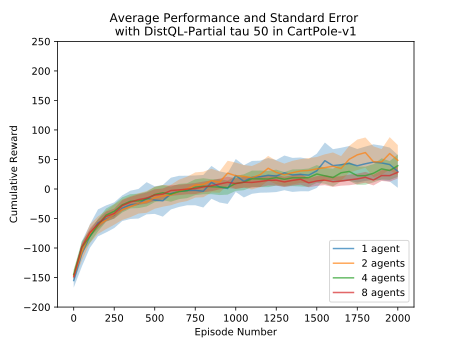
\includegraphics[width=0.7\linewidth]{resultImages/binned-Average-Performance-and-Standard-Error-with-DistQL-Partial-tau-50-in-CartPole-v1}
	\caption{}
	\label{fig:binned-Average-Performance-and-Standard-Error-with-DistQL-Partial-tau-50-in-CartPole-v1}
\end{figure}

\begin{figure}[h]
	\centering
	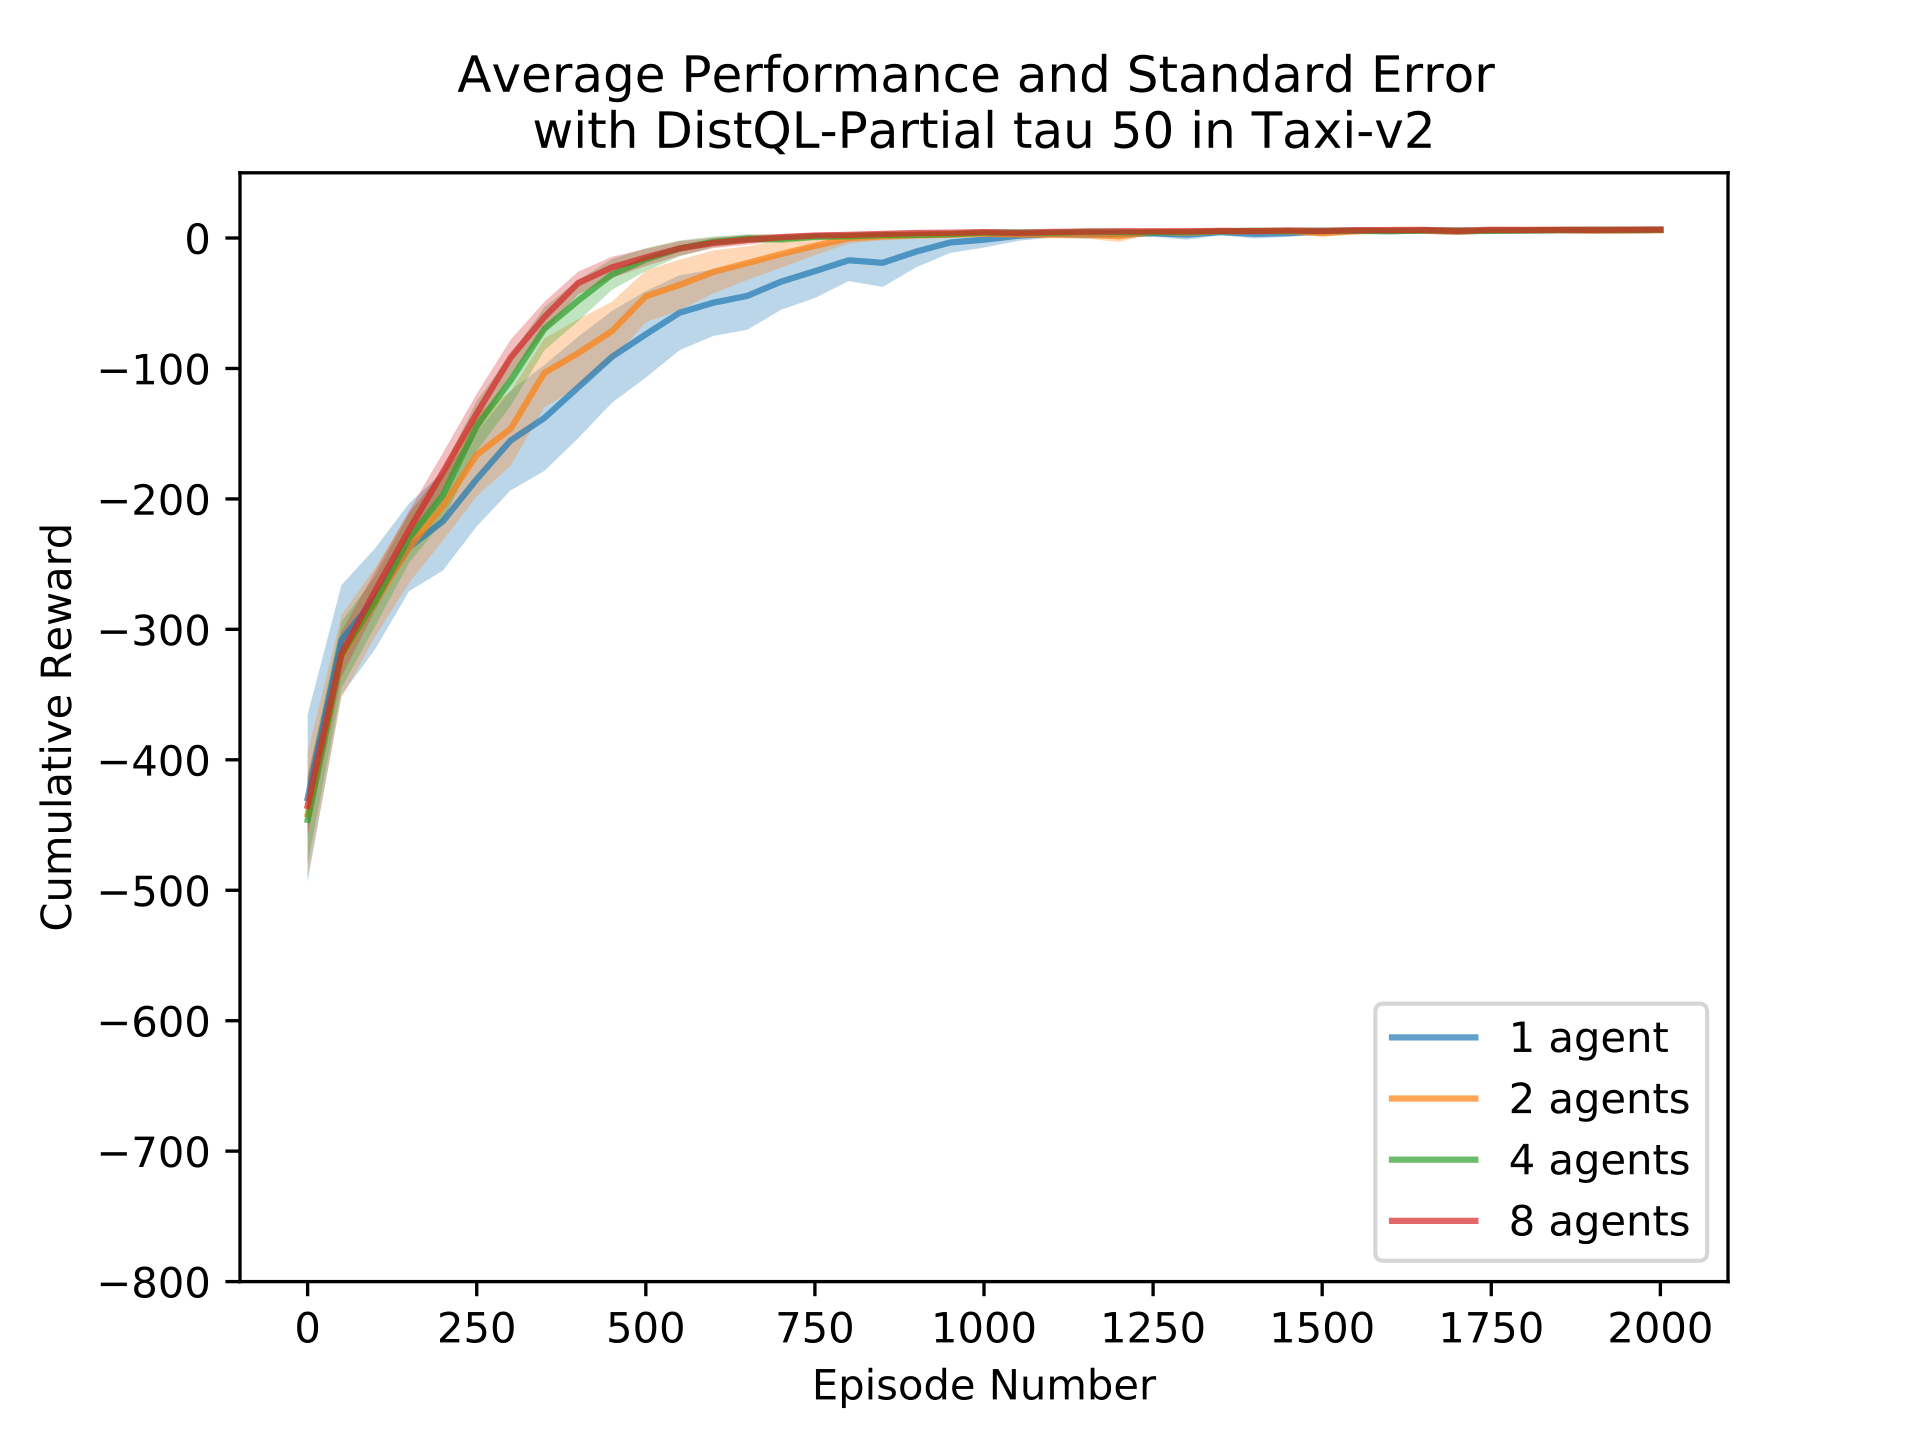
\includegraphics[width=0.7\linewidth]{resultImages/binned-Average-Performance-and-Standard-Error-with-DistQL-Partial-tau-50-in-Taxi-v2}
	\caption{}
	\label{fig:binned-Average-Performance-and-Standard-Error-with-DistQL-Partial-tau-50-in-Taxi-v2}
\end{figure}

\begin{figure}[h]
	\centering
	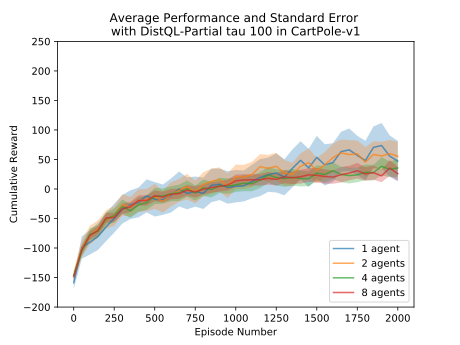
\includegraphics[width=0.7\linewidth]{resultImages/binned-Average-Performance-and-Standard-Error-with-DistQL-Partial-tau-100-in-CartPole-v1}
	\caption{}
	\label{fig:binned-Average-Performance-and-Standard-Error-with-DistQL-Partial-tau-100-in-CartPole-v1}
\end{figure}

\begin{figure}[h]
	\centering
	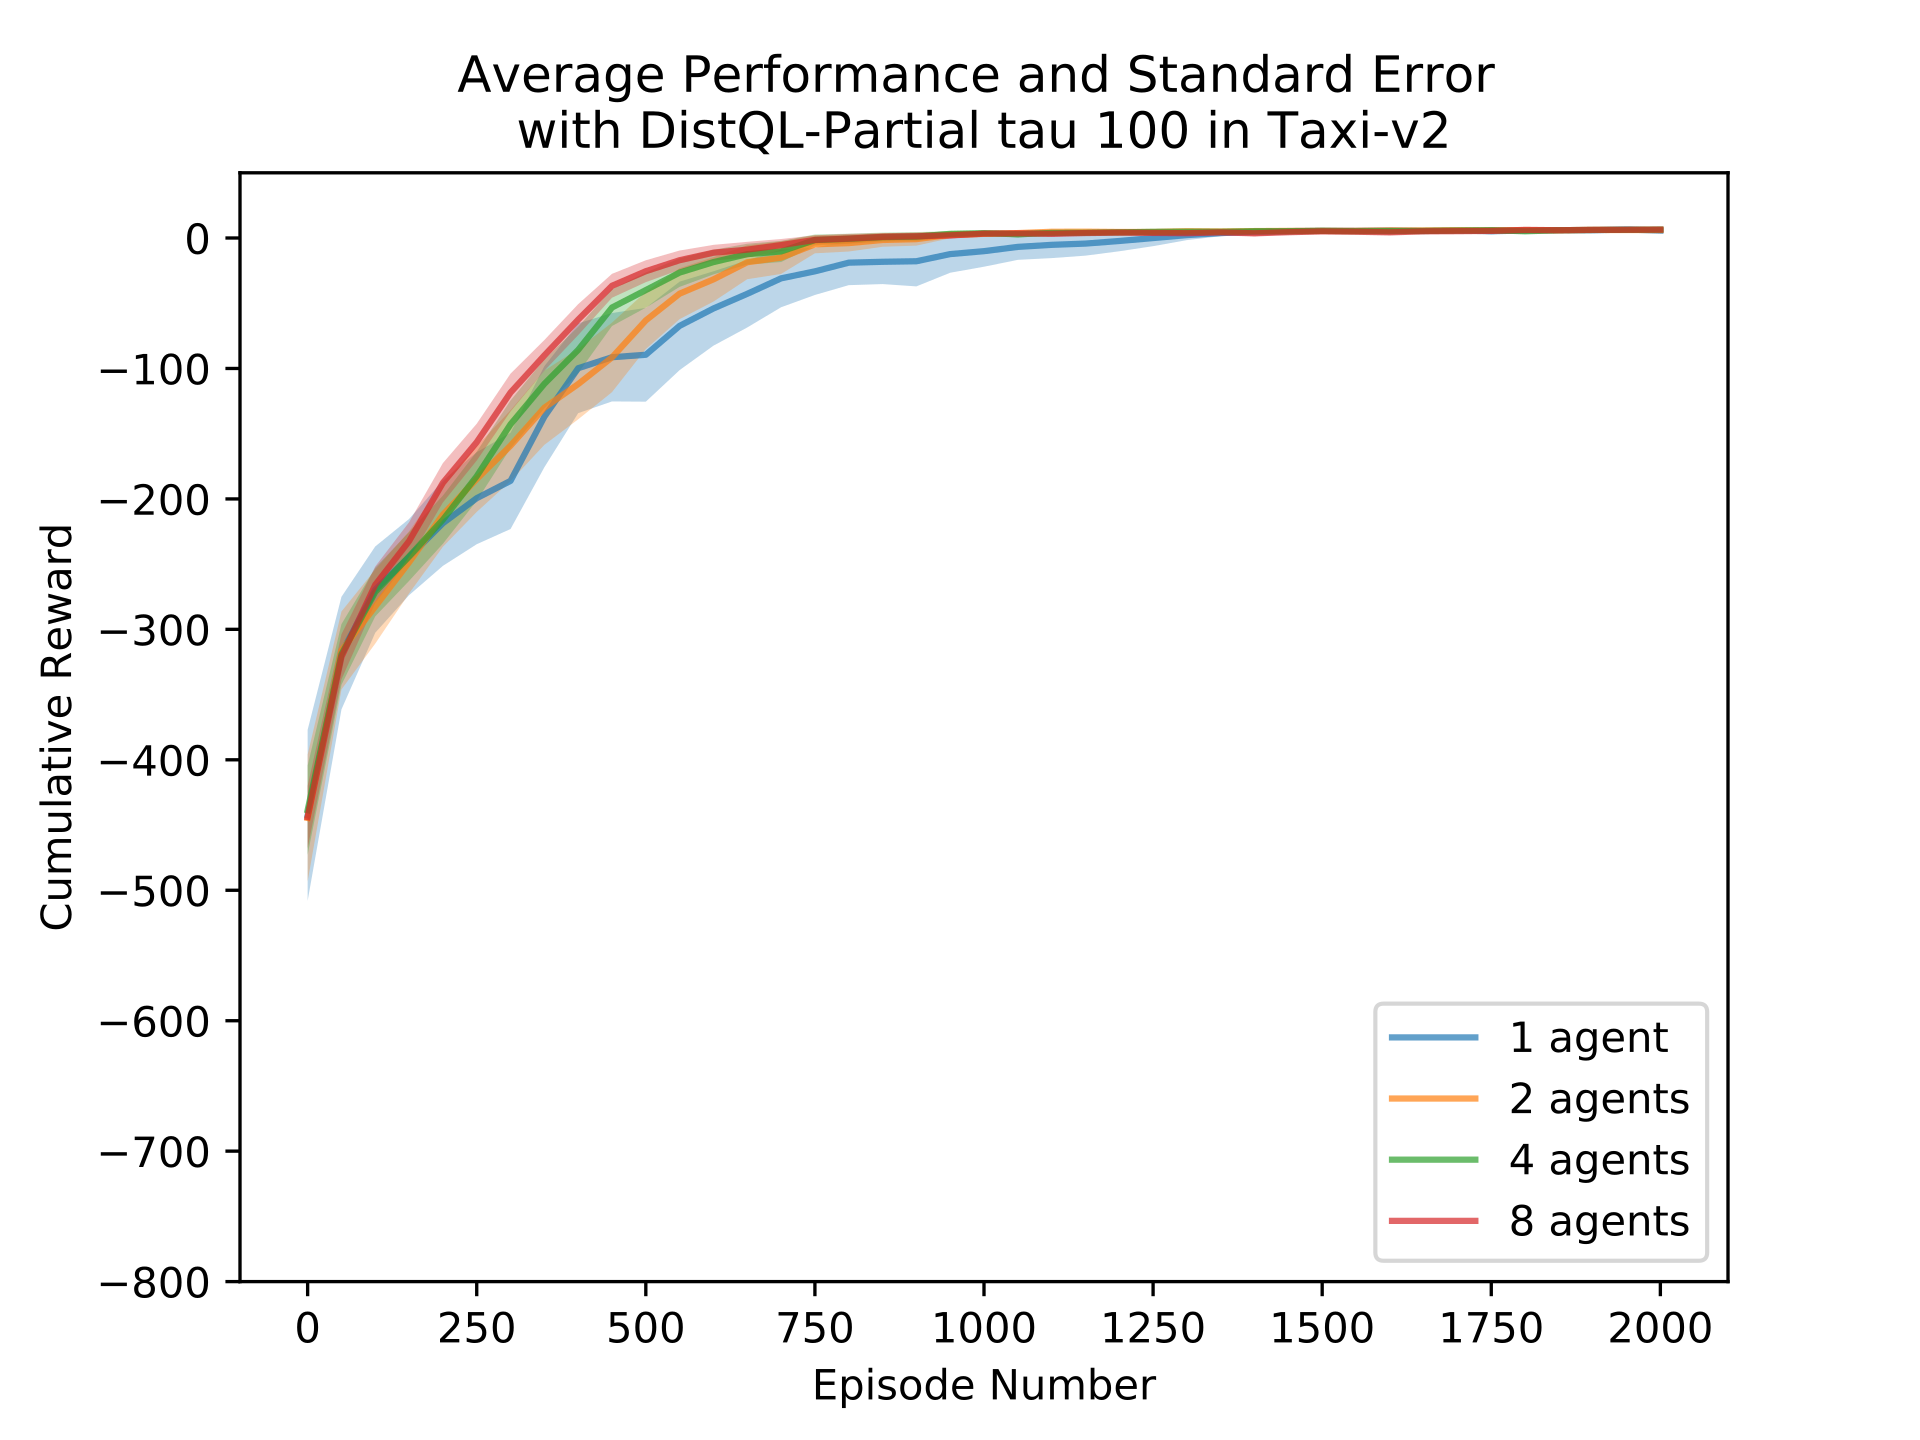
\includegraphics[width=0.7\linewidth]{resultImages/binned-Average-Performance-and-Standard-Error-with-DistQL-Partial-tau-100-in-Taxi-v2}
	\caption{}
	\label{fig:binned-Average-Performance-and-Standard-Error-with-DistQL-Partial-tau-100-in-Taxi-v2}
\end{figure}
\fi


%\section{Discussion}
%\label{discussion}

\section{Future Work}
\label{future}
DistQL opens the door for a host of other work to follow after and to build upon it. As a result, there are several interesting areas to explore for future work. 

The current implementation of DistQL uses an aggregation function that relies on a central learning rate to help arbitrate the updates of the different worker agents in an asynchronous manner. Future work could explore what other possible aggregation functions could be used instead. A possible example would be treating the learning rates as the likelihood of convergence to that Q-value. An expected value function could then be used to aggregate the Q-values for each agent. This could help remove additional hyperparameters from the learning process.

The asynchronous nature of DistQL is a bonus but was not formally shown to be optimal. Work has been done by Tsitsiklis (1994) \nocite{Tsitsiklis1994} showed Q-Learning can be optimal in an asynchronous setting. Future work to show if DistQL fits the guidelines that Tsitsiklis created could determine if aggregation techniques like those used in DistQL do or do not break the optimality guarantees of Q-Learning. 

The effect of different exploration strategies would also be of interest for future work. As shown by the DistQL-ALL to DistQL-Partial comparison, a large part of the power of DistQL-ALL comes from the shared exploration of worker agents. Using different exploration strategies or even different exploration strategies per worker and how they effected learning would be of significant interest. 

\section{Conclusion}
\label{conclusion}
This paper introduces the idea of Distributed Q-Learning using a centralized QServer. An aggregation function is described, and different versions of DistQL were shown to demonstrate the effect the effects of how updates occur and how the frequency of updates can effect learning. 

While more work needs to be done, experiments showed that it is possible to decrease the number of episodes needed for an agent to learn a good policy by distributing the learning process amongst several learners, aggregating the experiences, and distributing it back among them.

\vskip 0.2in
\bibliography{DistributedQLearning}
\bibliographystyle{theapa}

\end{document}






